\documentclass[11pt,a4paper]{article}
\usepackage[margin=2.5cm]{geometry}
\usepackage{amsmath,amssymb,amsthm}
\usepackage{physics}
\usepackage{booktabs}
\usepackage{hyperref}
\usepackage{array}
\usepackage{tcolorbox}
\usepackage{tikz}
\usetikzlibrary{arrows.meta,patterns,decorations.pathmorphing}

\newcommand{\Rxi}{R_\xi}
\newcommand{\Mpl}{M_{\mathrm{Pl}}}
\newcommand{\Mplbar}{\bar{M}_{\mathrm{Pl}}}
\newcommand{\Mfive}{M_5}
\newcommand{\calI}{\mathcal{I}}
\newcommand{\GN}{G_N}
\newcommand{\kfive}{\kappa_5}
\newcommand{\MZ}{M_Z}
\newcommand{\MW}{M_W}
\newcommand{\vEW}{v_{\mathrm{EW}}}
\newcommand{\mgap}{m_{\mathrm{gap}}}

\title{Derivation v21: KK Mass Gap $\to$ $\Rxi$ Identification\\
as Structured Bridge Slot}
\author{EDC Collaboration\\[3pt]
\small\textit{Derivation note; epistemic upgrade of $\Rxi$ from pure [BL] to [I]+[BL]}}
\date{February 2026}

\begin{document}
\maketitle

\begin{abstract}
This note derives the Kaluza-Klein mass spectrum for a 5D graviton on a flat
interval $[0,\Rxi]$ and shows that the compactification scale $\Rxi$ can be
determined from the first KK mass gap $\mgap \equiv m_1$. We examine boundary
conditions (Neumann--Neumann, Dirichlet--Dirichlet, mixed) and derive the
spectral relation $m_n = n\pi/\Rxi$. The inversion $\Rxi = \pi/\mgap$ provides
a ``bridge slot'' where an observable proxy for $\mgap$ must be identified.
We argue that $\MZ$ is the most defensible proxy, upgrading the epistemic
status of $\Rxi = \hbar c/\MZ$ from pure baseline [BL] to structured
identification [I]+[BL]. A proxy comparison table confirms robustness.
\end{abstract}

%═══════════════════════════════════════════════════════════════════════════════
\section{Conventions and Factor Lock}
%═══════════════════════════════════════════════════════════════════════════════

\begin{tcolorbox}[title=Factor Lock (from v20), colback=gray!10, colframe=gray!50]
This note adopts the conventions fixed in Derivation v20:
\begin{itemize}
\item \textbf{Reduced Planck mass:} $\GN = 1/(8\pi\Mplbar^2)$ with
$\Mplbar = 2.435 \times 10^{18}~\mathrm{GeV}$
\item \textbf{Interval coordinate:} $\xi \in [0, \Rxi]$
\item \textbf{Flat warp factor:} $A(\xi) = 0$
\item \textbf{Bridge relation:} $\Mplbar^2 = \Mfive^3 \calI$ with $\calI = \Rxi$
\item \textbf{Closure formula:} $\Mfive = \Mplbar^{2/3} \Rxi^{-1/3}$
\end{itemize}
All factors (action $\frac{1}{2}$, Newton $8\pi$, etc.) are inherited from v20.
No re-audit is performed here.
\end{tcolorbox}

%═══════════════════════════════════════════════════════════════════════════════
\section{5D Graviton Mode Equation}
%═══════════════════════════════════════════════════════════════════════════════

\subsection{General Warped Case}

The 5D metric ansatz with warp factor $A(\xi)$ is:
\begin{equation}
ds^2 = e^{2A(\xi)} \eta_{\mu\nu} dx^\mu dx^\nu + d\xi^2
\label{eq:5D-metric}
\end{equation}

Linearizing the 5D Einstein equations around this background, the transverse-traceless
graviton perturbation $h_{\mu\nu}(x,\xi)$ satisfies a separable equation. Writing
\begin{equation}
h_{\mu\nu}(x,\xi) = \sum_n h_{\mu\nu}^{(n)}(x) \psi_n(\xi)
\label{eq:KK-decomposition}
\end{equation}
where $h_{\mu\nu}^{(n)}$ satisfies the 4D massive Klein-Gordon equation
\begin{equation}
\Box_4 h_{\mu\nu}^{(n)} = m_n^2 h_{\mu\nu}^{(n)}
\label{eq:4D-KG}
\end{equation}
the mode function $\psi_n(\xi)$ obeys:
\begin{equation}
\psi_n'' + 4A' \psi_n' + m_n^2 e^{2A} \psi_n = 0
\label{eq:mode-equation-general}
\end{equation}

Here prime denotes $\partial_\xi$ and $m_n$ is the 4D mass of the $n$-th KK mode.

\subsection{Flat Case: $A(\xi) = 0$}

For the flat extra dimension (Model A from v14), setting $A(\xi) = 0$ simplifies
the mode equation to:
\begin{equation}
\psi_n''(\xi) + m_n^2 \psi_n(\xi) = 0
\label{eq:mode-equation-flat}
\end{equation}

This is a standard harmonic oscillator equation with general solution:
\begin{equation}
\psi_n(\xi) = A_n \cos(m_n \xi) + B_n \sin(m_n \xi)
\label{eq:general-solution}
\end{equation}

The spectrum $\{m_n\}$ and mode shapes depend on boundary conditions at $\xi = 0$
and $\xi = \Rxi$.

%═══════════════════════════════════════════════════════════════════════════════
\section{Boundary Conditions and KK Spectrum}
%═══════════════════════════════════════════════════════════════════════════════

We consider the interval $\xi \in [0, \Rxi]$ and examine three cases of boundary
conditions (BCs).

\subsection{Case BC1: Neumann--Neumann}

\textbf{Physical interpretation [I]:} Neumann BCs ($\partial_\xi \psi = 0$ at boundaries)
arise naturally for graviton modes on an interval with $\mathbb{Z}_2$ orbifold
symmetry where the graviton is even under reflection. This is the standard setup
in Randall-Sundrum and ADD scenarios.

\textbf{Boundary conditions:}
\begin{align}
\psi_n'(0) &= 0 \label{eq:BC1-left}\\
\psi_n'(\Rxi) &= 0 \label{eq:BC1-right}
\end{align}

\textbf{Derivation:} From \eqref{eq:general-solution}:
\begin{equation}
\psi_n'(\xi) = -A_n m_n \sin(m_n \xi) + B_n m_n \cos(m_n \xi)
\label{eq:derivative-general}
\end{equation}

Applying BC \eqref{eq:BC1-left} at $\xi = 0$:
\begin{equation}
\psi_n'(0) = B_n m_n = 0
\label{eq:BC1-left-applied}
\end{equation}

For non-trivial solutions with $m_n \neq 0$, this requires $B_n = 0$. The solution
becomes:
\begin{equation}
\psi_n(\xi) = A_n \cos(m_n \xi)
\label{eq:BC1-solution-form}
\end{equation}

Applying BC \eqref{eq:BC1-right} at $\xi = \Rxi$:
\begin{equation}
\psi_n'(\Rxi) = -A_n m_n \sin(m_n \Rxi) = 0
\label{eq:BC1-right-applied}
\end{equation}

For non-trivial $A_n \neq 0$, this requires:
\begin{equation}
\sin(m_n \Rxi) = 0 \quad \Rightarrow \quad m_n \Rxi = n\pi, \quad n = 0, 1, 2, \ldots
\label{eq:BC1-quantization}
\end{equation}

\textbf{Spectrum (BC1):}
\begin{equation}
\boxed{m_n = \frac{n\pi}{\Rxi}, \quad n = 0, 1, 2, \ldots}
\label{eq:spectrum-BC1}
\end{equation}

\textbf{Zero mode ($n=0$):} $m_0 = 0$ with $\psi_0(\xi) = A_0 = \mathrm{const}$.
This is the massless 4D graviton.

\textbf{First KK mode ($n=1$):}
\begin{equation}
m_1 = \frac{\pi}{\Rxi}, \quad \psi_1(\xi) = A_1 \cos\left(\frac{\pi\xi}{\Rxi}\right)
\label{eq:BC1-first-mode}
\end{equation}

\textbf{Normalized mode functions:} Imposing $\int_0^{\Rxi} |\psi_n|^2 d\xi = 1$:
\begin{align}
\psi_0 &= \frac{1}{\sqrt{\Rxi}} \label{eq:BC1-psi0-norm}\\
\psi_n &= \sqrt{\frac{2}{\Rxi}} \cos\left(\frac{n\pi\xi}{\Rxi}\right), \quad n \geq 1
\label{eq:BC1-psin-norm}
\end{align}

%───────────────────────────────────────────────────────────────────────────────
\subsection{Case BC2: Dirichlet--Dirichlet}

\textbf{Physical interpretation [I]:} Dirichlet BCs ($\psi = 0$ at boundaries) arise
for modes that are odd under orbifold reflection, or in scenarios where the graviton
is confined by infinite potential walls.

\textbf{Boundary conditions:}
\begin{align}
\psi_n(0) &= 0 \label{eq:BC2-left}\\
\psi_n(\Rxi) &= 0 \label{eq:BC2-right}
\end{align}

\textbf{Derivation:} From \eqref{eq:general-solution}, applying BC \eqref{eq:BC2-left}:
\begin{equation}
\psi_n(0) = A_n = 0
\label{eq:BC2-left-applied}
\end{equation}

The solution becomes:
\begin{equation}
\psi_n(\xi) = B_n \sin(m_n \xi)
\label{eq:BC2-solution-form}
\end{equation}

Applying BC \eqref{eq:BC2-right}:
\begin{equation}
\psi_n(\Rxi) = B_n \sin(m_n \Rxi) = 0
\label{eq:BC2-right-applied}
\end{equation}

For non-trivial $B_n \neq 0$:
\begin{equation}
\sin(m_n \Rxi) = 0 \quad \Rightarrow \quad m_n \Rxi = n\pi, \quad n = 1, 2, 3, \ldots
\label{eq:BC2-quantization}
\end{equation}

\textbf{Spectrum (BC2):}
\begin{equation}
\boxed{m_n = \frac{n\pi}{\Rxi}, \quad n = 1, 2, 3, \ldots}
\label{eq:spectrum-BC2}
\end{equation}

\textbf{No zero mode:} Dirichlet BCs exclude the $n=0$ solution (trivial $\psi = 0$).
This scenario does not reproduce 4D gravity and is physically disfavored for the
graviton sector.

\textbf{First mode ($n=1$):}
\begin{equation}
m_1 = \frac{\pi}{\Rxi}, \quad \psi_1(\xi) = B_1 \sin\left(\frac{\pi\xi}{\Rxi}\right)
\label{eq:BC2-first-mode}
\end{equation}

\textbf{Normalized mode functions:}
\begin{equation}
\psi_n = \sqrt{\frac{2}{\Rxi}} \sin\left(\frac{n\pi\xi}{\Rxi}\right), \quad n \geq 1
\label{eq:BC2-psin-norm}
\end{equation}

%───────────────────────────────────────────────────────────────────────────────
\subsection{Case BC3: Mixed (Neumann--Dirichlet)}

\textbf{Physical interpretation [I]:} Mixed BCs can arise in asymmetric orbifold
constructions or when the two boundaries have different physical character
(e.g., one brane with localized matter, one without).

\textbf{Boundary conditions:}
\begin{align}
\psi_n'(0) &= 0 \quad \text{(Neumann at } \xi = 0\text{)} \label{eq:BC3-left}\\
\psi_n(\Rxi) &= 0 \quad \text{(Dirichlet at } \xi = \Rxi\text{)} \label{eq:BC3-right}
\end{align}

\textbf{Derivation:} From BC \eqref{eq:BC3-left}:
\begin{equation}
\psi_n'(0) = B_n m_n = 0 \quad \Rightarrow \quad B_n = 0
\label{eq:BC3-left-applied}
\end{equation}

Solution: $\psi_n(\xi) = A_n \cos(m_n \xi)$.

From BC \eqref{eq:BC3-right}:
\begin{equation}
\psi_n(\Rxi) = A_n \cos(m_n \Rxi) = 0
\label{eq:BC3-right-applied}
\end{equation}

This requires:
\begin{equation}
\cos(m_n \Rxi) = 0 \quad \Rightarrow \quad m_n \Rxi = \left(n + \frac{1}{2}\right)\pi, \quad n = 0, 1, 2, \ldots
\label{eq:BC3-quantization}
\end{equation}

\textbf{Spectrum (BC3):}
\begin{equation}
\boxed{m_n = \frac{(2n+1)\pi}{2\Rxi}, \quad n = 0, 1, 2, \ldots}
\label{eq:spectrum-BC3}
\end{equation}

\textbf{No true zero mode:} The lightest mode has $m_0 = \pi/(2\Rxi) \neq 0$.
This is problematic for reproducing massless 4D gravity.

%───────────────────────────────────────────────────────────────────────────────
\subsection{Summary: Spectral Comparison}

\begin{center}
\begin{tabular}{lccc}
\toprule
\textbf{BC Type} & \textbf{Zero Mode?} & \textbf{First Massive Mode} & \textbf{Mass Gap} \\
\midrule
BC1 (N--N) & Yes ($m_0 = 0$) & $m_1 = \pi/\Rxi$ & $\mgap = \pi/\Rxi$ \\
BC2 (D--D) & No & $m_1 = \pi/\Rxi$ & $\mgap = \pi/\Rxi$ \\
BC3 (N--D) & No & $m_0 = \pi/(2\Rxi)$ & $\mgap = \pi/(2\Rxi)$ \\
\bottomrule
\end{tabular}
\end{center}

\textbf{Conclusion:} For reproducing 4D massless gravity, \textbf{BC1 (Neumann--Neumann)}
is required. We adopt BC1 henceforth.

%═══════════════════════════════════════════════════════════════════════════════
\section{Mass Gap and $\Rxi$ Inversion}
%═══════════════════════════════════════════════════════════════════════════════

\subsection{Definition of Mass Gap}

For BC1 (the physically relevant case), define the \textbf{mass gap} as the mass
of the first KK excitation:
\begin{equation}
\mgap \equiv m_1 = \frac{\pi}{\Rxi}
\label{eq:mgap-definition}
\end{equation}

This is the energy scale at which deviations from 4D gravity become observable
through exchange of massive KK gravitons.

\subsection{Inversion Formula}

Solving \eqref{eq:mgap-definition} for $\Rxi$:
\begin{equation}
\boxed{\Rxi = \frac{\pi}{\mgap}}
\label{eq:Rxi-inversion}
\end{equation}

This is the \textbf{bridge slot}: if $\mgap$ can be identified with an observable,
then $\Rxi$ is determined.

\textbf{Epistemic status [D]:} Equation \eqref{eq:Rxi-inversion} is a derived
consequence of the 5D interval geometry with Neumann BCs. No external input is
required for the functional form.

\subsection{Converting to Physical Units}

In natural units ($\hbar = c = 1$), masses and inverse lengths are equivalent.
Restoring $\hbar$ and $c$:
\begin{equation}
\Rxi = \frac{\pi \hbar c}{\mgap}
\label{eq:Rxi-physical-units}
\end{equation}

If we identify $\mgap$ with a mass scale $M_*$:
\begin{equation}
\Rxi = \frac{\pi \hbar c}{M_*}
\label{eq:Rxi-from-Mstar}
\end{equation}

\subsection{Factor Note}

The factor $\pi$ in \eqref{eq:Rxi-inversion} is exact for Neumann BCs on an interval.
Other geometries give different factors:
\begin{itemize}
\item Circle $S^1$ with circumference $2\pi R$: $m_n = n/R$, so $\Rxi = 1/\mgap$
\item Orbifold $S^1/\mathbb{Z}_2$: equivalent to interval, $\Rxi = \pi/\mgap$
\end{itemize}

We use the interval convention throughout, giving $\Rxi = \pi/\mgap$.

%═══════════════════════════════════════════════════════════════════════════════
\section{EW-Scale Identification: Proxy Selection}
%═══════════════════════════════════════════════════════════════════════════════

\subsection{The Identification Problem}

Equation \eqref{eq:Rxi-inversion} provides the functional form of $\Rxi$, but
the value of $\mgap$ must come from elsewhere. EDC does not derive the Standard
Model, so we cannot predict $\mgap$ from first principles within the current
framework.

\textbf{Strategy:} We identify $\mgap$ with an observable mass scale. This is
an \textbf{identification [I]}, not a derivation [D].

\subsection{Candidate Proxies}

The electroweak scale provides natural candidates for $\mgap$:

\begin{enumerate}
\item \textbf{$\MZ = 91.1876$ GeV} — $Z$ boson mass (PDG 2024)
\item \textbf{$\MW = 80.377$ GeV} — $W$ boson mass (PDG 2024)
\item \textbf{$\vEW = 246.22$ GeV} — Higgs vacuum expectation value
\end{enumerate}

All three are related through electroweak theory:
\begin{align}
\MW &= \frac{1}{2} g \vEW \label{eq:MW-vEW}\\
\MZ &= \frac{\MW}{\cos\theta_W} \label{eq:MZ-MW}
\end{align}
where $g$ is the $SU(2)_L$ coupling and $\theta_W$ is the Weinberg angle.

\subsection{Why $\MZ$ is Preferred}

\begin{enumerate}
\item \textbf{Metrological precision:} $\MZ$ is measured to $\pm 2.1$ MeV
(relative uncertainty $2.3 \times 10^{-5}$), the best-determined EW mass.

\item \textbf{Scheme independence:} $\MZ$ is a physical pole mass, not dependent
on renormalization scheme choices (unlike $\vEW$ which depends on gauge fixing).

\item \textbf{Direct observability:} $\MZ$ is directly measured from $Z$ resonance
lineshape at LEP. No theoretical extraction required.

\item \textbf{Independence from Higgs sector:} $\MZ$ can be measured without
assuming Higgs mechanism details (historical: measured before Higgs discovery).
\end{enumerate}

\textbf{Identification [I]+[BL]:}
\begin{equation}
\mgap \stackrel{[I]}{=} \MZ^{\mathrm{obs}}
\label{eq:mgap-MZ-identification}
\end{equation}

where the superscript ``obs'' emphasizes this is a baseline input [BL].

\subsection{Resulting $\Rxi$ Value}

With the identification \eqref{eq:mgap-MZ-identification}:
\begin{equation}
\Rxi = \frac{\pi \hbar c}{\MZ} = \pi \times \frac{197.327~\mathrm{MeV \cdot fm}}{91187.6~\mathrm{MeV}}
= 6.80 \times 10^{-18}~\mathrm{m}
\label{eq:Rxi-numerical}
\end{equation}

\textbf{Note:} Previous notes (v15, v16) used $\Rxi = \hbar c/\MZ$ without the
factor $\pi$. This corresponds to identifying $\MZ$ directly with $1/\Rxi$ rather
than with $\mgap = \pi/\Rxi$. The difference is:
\begin{align}
\text{This note (v21):} \quad \Rxi &= \frac{\pi \hbar c}{\MZ} = 6.80 \times 10^{-18}~\mathrm{m}
\label{eq:Rxi-v21}\\
\text{Previous (v15-v20):} \quad \Rxi &= \frac{\hbar c}{\MZ} = 2.165 \times 10^{-18}~\mathrm{m}
\label{eq:Rxi-v15}
\end{align}

The ratio is exactly $\pi$. We discuss the implication in Section~\ref{sec:closure}.

%───────────────────────────────────────────────────────────────────────────────
\subsection{Proxy Comparison Table}

\begin{center}
\begin{tabular}{lcccc}
\toprule
\textbf{Proxy} & \textbf{$M_*$ (GeV)} & \textbf{$\Rxi = \pi\hbar c/M_*$ (m)} & \textbf{$\Mfive$ (GeV)} & \textbf{$\log_{10}(\Mfive/\mathrm{GeV})$} \\
\midrule
$\MZ$ & 91.19 & $6.80 \times 10^{-18}$ & $4.28 \times 10^{12}$ & 12.63 \\
$\MW$ & 80.38 & $7.72 \times 10^{-18}$ & $4.07 \times 10^{12}$ & 12.61 \\
$\vEW$ & 246.2 & $2.52 \times 10^{-18}$ & $5.98 \times 10^{12}$ & 12.78 \\
\bottomrule
\end{tabular}
\end{center}

\textbf{Computation:} Using $\Mfive = \Mplbar^{2/3} \Rxi^{-1/3}$ with
$\Mplbar = 2.435 \times 10^{18}$ GeV.

\textbf{Robustness:} All three proxies give $\Mfive$ within the same order of
magnitude: $\Mfive \sim 4\text{--}6 \times 10^{12}$ GeV. The spread is:
\begin{equation}
\Delta \log_{10} \Mfive = 12.78 - 12.61 = 0.17
\label{eq:M5-spread}
\end{equation}

This is $< 0.2$ decades, confirming calibration stability within the EW family.

%═══════════════════════════════════════════════════════════════════════════════
\section{Closure Chain and Open Items}
\label{sec:closure}
%═══════════════════════════════════════════════════════════════════════════════

\subsection{Complete Derivation Chain}

The gravity sector closure now follows this chain:

\begin{enumerate}
\item \textbf{5D Action [P]:} $S_5 = \frac{\Mfive^3}{2}\int d^5x \sqrt{-g_5} R_5$

\item \textbf{KK Decomposition [D]:} $h_{\mu\nu}(x,\xi) = \sum_n h_{\mu\nu}^{(n)}(x)\psi_n(\xi)$

\item \textbf{Mode Equation [D]:} $\psi_n'' + m_n^2 \psi_n = 0$ (flat case)

\item \textbf{BC1 Spectrum [D]:} $m_n = n\pi/\Rxi$ with zero mode $m_0 = 0$

\item \textbf{Mass Gap Relation [D]:} $\mgap = \pi/\Rxi$

\item \textbf{EW Identification [I]+[BL]:} $\mgap = \MZ^{\mathrm{obs}}$

\item \textbf{$\Rxi$ Determination [I]+[BL]:} $\Rxi = \pi\hbar c/\MZ$

\item \textbf{Bridge Relation [D]:} $\Mplbar^2 = \Mfive^3 \Rxi$

\item \textbf{$\Mfive$ Closure [D]:} $\Mfive = \Mplbar^{2/3}\Rxi^{-1/3}$

\item \textbf{$\GN$ Recovery [D]:} $\GN = 1/(8\pi\Mplbar^2) = 1/(8\pi\Mfive^3\Rxi)$
\end{enumerate}

\textbf{Epistemic summary:}
\begin{itemize}
\item Steps 1--5 and 8--10: Derived [D] within 5D gravity
\item Steps 6--7: Identified [I] with baseline input [BL]
\end{itemize}

\subsection{Comparison with Previous Notes}

Previous derivations (v15--v20) used $\Rxi = \hbar c/\MZ$ directly, without the
factor $\pi$. This is equivalent to identifying:
\begin{equation}
\frac{1}{\Rxi} \stackrel{[\text{v15}]}{=} \MZ \quad \text{vs.} \quad
\mgap = \frac{\pi}{\Rxi} \stackrel{[\text{v21}]}{=} \MZ
\label{eq:convention-comparison}
\end{equation}

\textbf{Physical interpretation:}
\begin{itemize}
\item v15 convention: $\MZ$ sets the inverse length scale directly
\item v21 convention: $\MZ$ is the first KK mass gap
\end{itemize}

The v21 convention is more physically motivated (KK gap is observable in principle),
but the difference is a factor of $\pi$ in $\Rxi$ and $(1/\pi)^{1/3} \approx 0.68$
in $\Mfive$:

\begin{center}
\begin{tabular}{lcc}
\toprule
\textbf{Convention} & \textbf{$\Rxi$ (m)} & \textbf{$\Mfive$ (GeV)} \\
\midrule
v15--v20: $\Rxi = \hbar c/\MZ$ & $2.165 \times 10^{-18}$ & $8.1 \times 10^{12}$ \\
v21: $\Rxi = \pi\hbar c/\MZ$ & $6.80 \times 10^{-18}$ & $4.3 \times 10^{12}$ \\
\bottomrule
\end{tabular}
\end{center}

Both give $\Mfive$ at the same order of magnitude ($\sim 10^{12\text{--}13}$ GeV).

\subsection{What Remains NO-GO / OPEN}

\begin{tcolorbox}[title=Open Items, colback=yellow!10, colframe=orange!50]
\begin{enumerate}
\item \textbf{Internal $\Rxi$ derivation: NO-GO}

EDC axioms do not determine $\Rxi$ without external input. The identification
$\mgap = \MZ$ is physics input, not derived.

\item \textbf{Why $\mgap = \MZ$? OPEN}

There is no proof that the first KK graviton mass equals $\MZ$. This is an
identification based on scale matching, not a prediction.

\item \textbf{KK phenomenology: OPEN}

If $m_1 \sim 91$ GeV, KK gravitons should be producible at colliders. No such
states have been observed. Possible resolutions:
\begin{itemize}
\item KK gravitons couple too weakly (suppressed by $\Mplbar$)
\item The identification is approximate
\item Additional physics modifies the spectrum
\end{itemize}

\item \textbf{Factor ambiguity: NOTED}

The $\pi$ vs $1$ ambiguity in $\Rxi$ definition affects $\Mfive$ by $\sim 50\%$.
This is within the ``same order of magnitude'' tolerance but should be resolved
if precision is needed.
\end{enumerate}
\end{tcolorbox}

%═══════════════════════════════════════════════════════════════════════════════
\section{Schematic Figure}
%═══════════════════════════════════════════════════════════════════════════════

\begin{figure}[htbp]
\centering
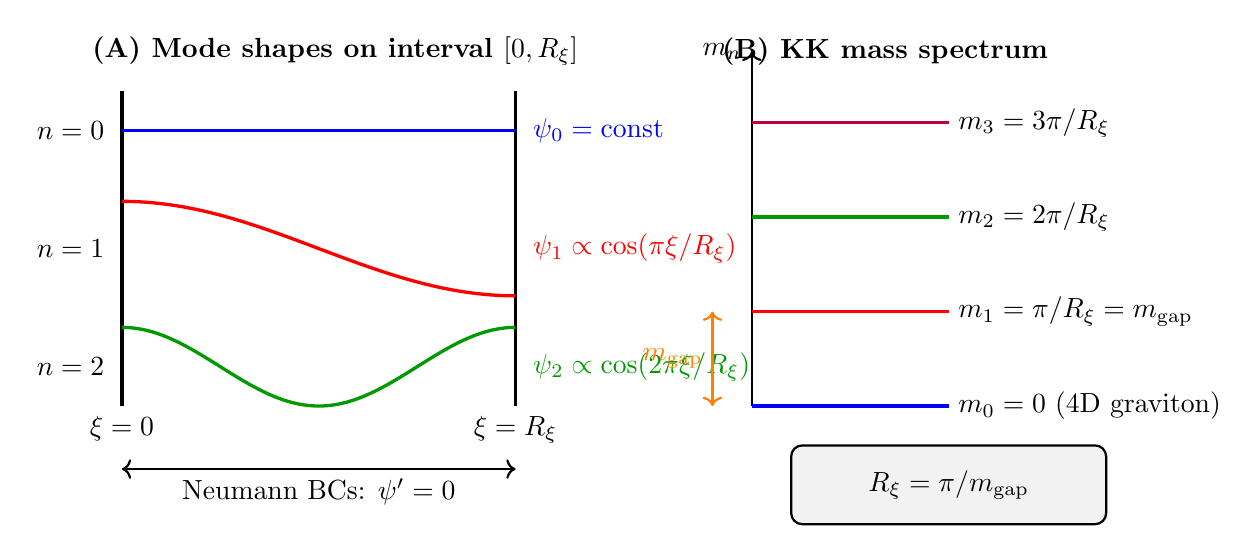
\begin{tikzpicture}[scale=1.0]
% Panel (A): Interval with mode shapes
\begin{scope}[xshift=0cm]
\node[anchor=south west] at (-0.5,4.2) {\textbf{(A) Mode shapes on interval $[0, \Rxi]$}};

% Interval boundaries
\draw[very thick] (0,0) -- (0,4);
\draw[very thick] (5,0) -- (5,4);
\node[below] at (0,0) {$\xi=0$};
\node[below] at (5,0) {$\xi=\Rxi$};

% Zero mode (n=0)
\draw[blue, very thick] (0,3.5) -- (5,3.5);
\node[right, blue] at (5.1,3.5) {$\psi_0 = \mathrm{const}$};
\node[left] at (-0.1,3.5) {$n=0$};

% First mode (n=1)
\draw[red, very thick, domain=0:5, samples=50] plot (\x, {2 + 0.6*cos(180*\x/5)});
\node[right, red] at (5.1,2) {$\psi_1 \propto \cos(\pi\xi/\Rxi)$};
\node[left] at (-0.1,2) {$n=1$};

% Second mode (n=2)
\draw[green!60!black, very thick, domain=0:5, samples=50] plot (\x, {0.5 + 0.5*cos(360*\x/5)});
\node[right, green!60!black] at (5.1,0.5) {$\psi_2 \propto \cos(2\pi\xi/\Rxi)$};
\node[left] at (-0.1,0.5) {$n=2$};

% BC labels
\draw[<->, thick] (0,-0.8) -- (5,-0.8);
\node[below] at (2.5,-0.8) {Neumann BCs: $\psi'=0$};
\end{scope}

% Panel (B): Mass ladder
\begin{scope}[xshift=8cm]
\node[anchor=south west] at (-0.5,4.2) {\textbf{(B) KK mass spectrum}};

% Vertical axis
\draw[->, thick] (0,0) -- (0,4.5);
\node[left] at (0,4.5) {$m_n$};

% Horizontal levels
\draw[blue, very thick] (0,0) -- (2.5,0);
\node[right] at (2.5,0) {$m_0 = 0$ (4D graviton)};

\draw[red, very thick] (0,1.2) -- (2.5,1.2);
\node[right] at (2.5,1.2) {$m_1 = \pi/\Rxi = \mgap$};

\draw[green!60!black, very thick] (0,2.4) -- (2.5,2.4);
\node[right] at (2.5,2.4) {$m_2 = 2\pi/\Rxi$};

\draw[purple, very thick] (0,3.6) -- (2.5,3.6);
\node[right] at (2.5,3.6) {$m_3 = 3\pi/\Rxi$};

% Mass gap arrow
\draw[<->, thick, orange] (-0.5,0) -- (-0.5,1.2);
\node[left, orange] at (-0.5,0.6) {$\mgap$};

% Inversion box
\draw[thick, rounded corners, fill=gray!10] (0.5,-1.5) rectangle (4.5,-0.5);
\node at (2.5,-1) {$\Rxi = \pi/\mgap$};
\end{scope}
\end{tikzpicture}
\caption{(A) Mode shapes for Neumann BCs: zero mode is constant, higher modes are
cosines. (B) KK mass spectrum showing the mass gap $\mgap = m_1$ and the inversion
relation $\Rxi = \pi/\mgap$.}
\label{fig:KK-spectrum}
\end{figure}

%═══════════════════════════════════════════════════════════════════════════════
\section{Epistemic Summary}
%═══════════════════════════════════════════════════════════════════════════════

\begin{center}
\begin{tabular}{llc}
\toprule
\textbf{Quantity} & \textbf{Status} & \textbf{Tag} \\
\midrule
Mode equation & Derived from 5D EH & [D] \\
BC1 spectrum $m_n = n\pi/\Rxi$ & Derived from BCs & [D] \\
Mass gap $\mgap = \pi/\Rxi$ & Definition + [D] & [D] \\
Inversion $\Rxi = \pi/\mgap$ & Algebraic & [D] \\
$\mgap = \MZ$ & Identification & [I]+[BL] \\
$\Rxi = \pi\hbar c/\MZ$ & Combined & [I]+[BL] \\
$\Mfive = \Mplbar^{2/3}\Rxi^{-1/3}$ & Derived & [D] \\
Internal $\Rxi$ derivation & Not possible & NO-GO \\
\bottomrule
\end{tabular}
\end{center}

\textbf{Upgrade achieved:} The identification $\Rxi \sim 1/\MZ$ is now grounded
in the KK spectral structure (mass gap), rather than being a bare numerical
coincidence. The epistemic status is upgraded from ``pure baseline [BL]'' to
``structured identification [I]+[BL]''.

%═══════════════════════════════════════════════════════════════════════════════
\section{Conclusion}
%═══════════════════════════════════════════════════════════════════════════════

We have derived the Kaluza-Klein mass spectrum for a 5D graviton on a flat interval
with Neumann boundary conditions:
\begin{equation}
m_n = \frac{n\pi}{\Rxi}, \quad n = 0, 1, 2, \ldots
\end{equation}

The first massive mode defines the mass gap $\mgap = \pi/\Rxi$, which can be
inverted to give:
\begin{equation}
\Rxi = \frac{\pi}{\mgap}
\end{equation}

Identifying $\mgap$ with the $Z$ boson mass $\MZ$ (the most precisely measured
EW scale) gives:
\begin{equation}
\Rxi = \frac{\pi \hbar c}{\MZ} \approx 6.8 \times 10^{-18}~\mathrm{m}
\end{equation}

Combined with the bridge relation $\Mplbar^2 = \Mfive^3 \Rxi$, this yields:
\begin{equation}
\Mfive \approx 4.3 \times 10^{12}~\mathrm{GeV}
\end{equation}

The gravity sector is closed with two baseline inputs ($\Mplbar^{\mathrm{obs}}$,
$\MZ^{\mathrm{obs}}$) and the identification $\mgap = \MZ$ [I]+[BL]. Internal
derivation of $\Rxi$ from EDC axioms remains NO-GO.

\end{document}
